\documentclass{article}
\usepackage{pgfplots}
\pgfplotsset{compat=1.17}

\begin{document}

\begin{tikzpicture}
    \begin{axis}[
        title={Coalescence times},
        xlabel={$\beta$},
        ylabel={$\mathbb{E}[T_{2}]$},
        xmin=0, xmax=1,
        ymin=0, ymax=15,
        xtick={0.2, 0.4, 0.6, 0.8, 1.0},
        ytick={0, 5, 10, 15},
        legend pos=south east,
        width=\textwidth,
        height=0.8\textheight,
        legend style={at={(0.5,-0.1)}, anchor=north,legend columns=-1},
        ]
        \addplot[black, thick] table {
            0.1 15
            0.2 5
            0.3 3
            0.4 2
            0.5 1
            0.6 1
            0.7 2
            0.8 5
            0.9 7
            1.0 7
        };
        \addlegendentry{Simulated ($N = 10^3$)}
        \addplot[green, thick] {15/(1+10*exp(-10*x))};
        \addlegendentry{Theoretic}
    \end{axis}
\end{tikzpicture}

\begin{tikzpicture}
    \begin{axis}[
        title={Strong selection},
        xlabel={$\beta$},
        ylabel={$v_N$},
        xmin=0, xmax=1,
        ymin=-3, ymax=2,
        xtick={0.2, 0.4, 0.6, 0.8, 1.0},
        ytick={-3, -2, -1, 0, 1, 2},
        legend pos=south east,
        width=\textwidth,
        height=0.8\textheight,
        legend style={at={(0.5,-0.1)}, anchor=north,legend columns=-1},
        ]
        \addplot[black, thick] table {
            0.1 -3
            0.2 -2
            0.3 -1
            0.4 0
            0.5 1
            0.6 2
            0.7 1
            0.8 0
            0.9 -1
            1.0 -2
        };
        \addlegendentry{Simulated ($N = 10^3$)}
        \addplot[green, thick] {15/(1+10*exp(-10*x))};
        \addlegendentry{Theoretic}
    \end{axis}
\end{tikzpicture}

\end{document}